\subsection{bpminterface/bpm\_\-interface.h File Reference}
\label{bpm__interface_8h}\index{bpminterface/bpm\_\-interface.h@{bpminterface/bpm\_\-interface.h}}


\subsubsection{Detailed Description}
Front end interface structure definitions and handlers. 

This header contains the front-end interface structures and handlers for libbpm. They define a set of user friendly structures like bpmconf\_\-t, bpmcalib\_\-t, beamconf\_\-t etc... to work with the bpm data. 

Definition in file {\bf bpm\_\-interface.h}.

{\tt \#include $<$stdio.h$>$}\par
{\tt \#include $<$stdlib.h$>$}\par
{\tt \#include $<$string.h$>$}\par
{\tt \#include $<$bpm/bpm\_\-defs.h$>$}\par
{\tt \#include $<$bpm/bpm\_\-wf.h$>$}\par
{\tt \#include $<$bpm/bpm\_\-dsp.h$>$}\par


Include dependency graph for bpm\_\-interface.h:\nopagebreak
\begin{figure}[H]
\begin{center}
\leavevmode
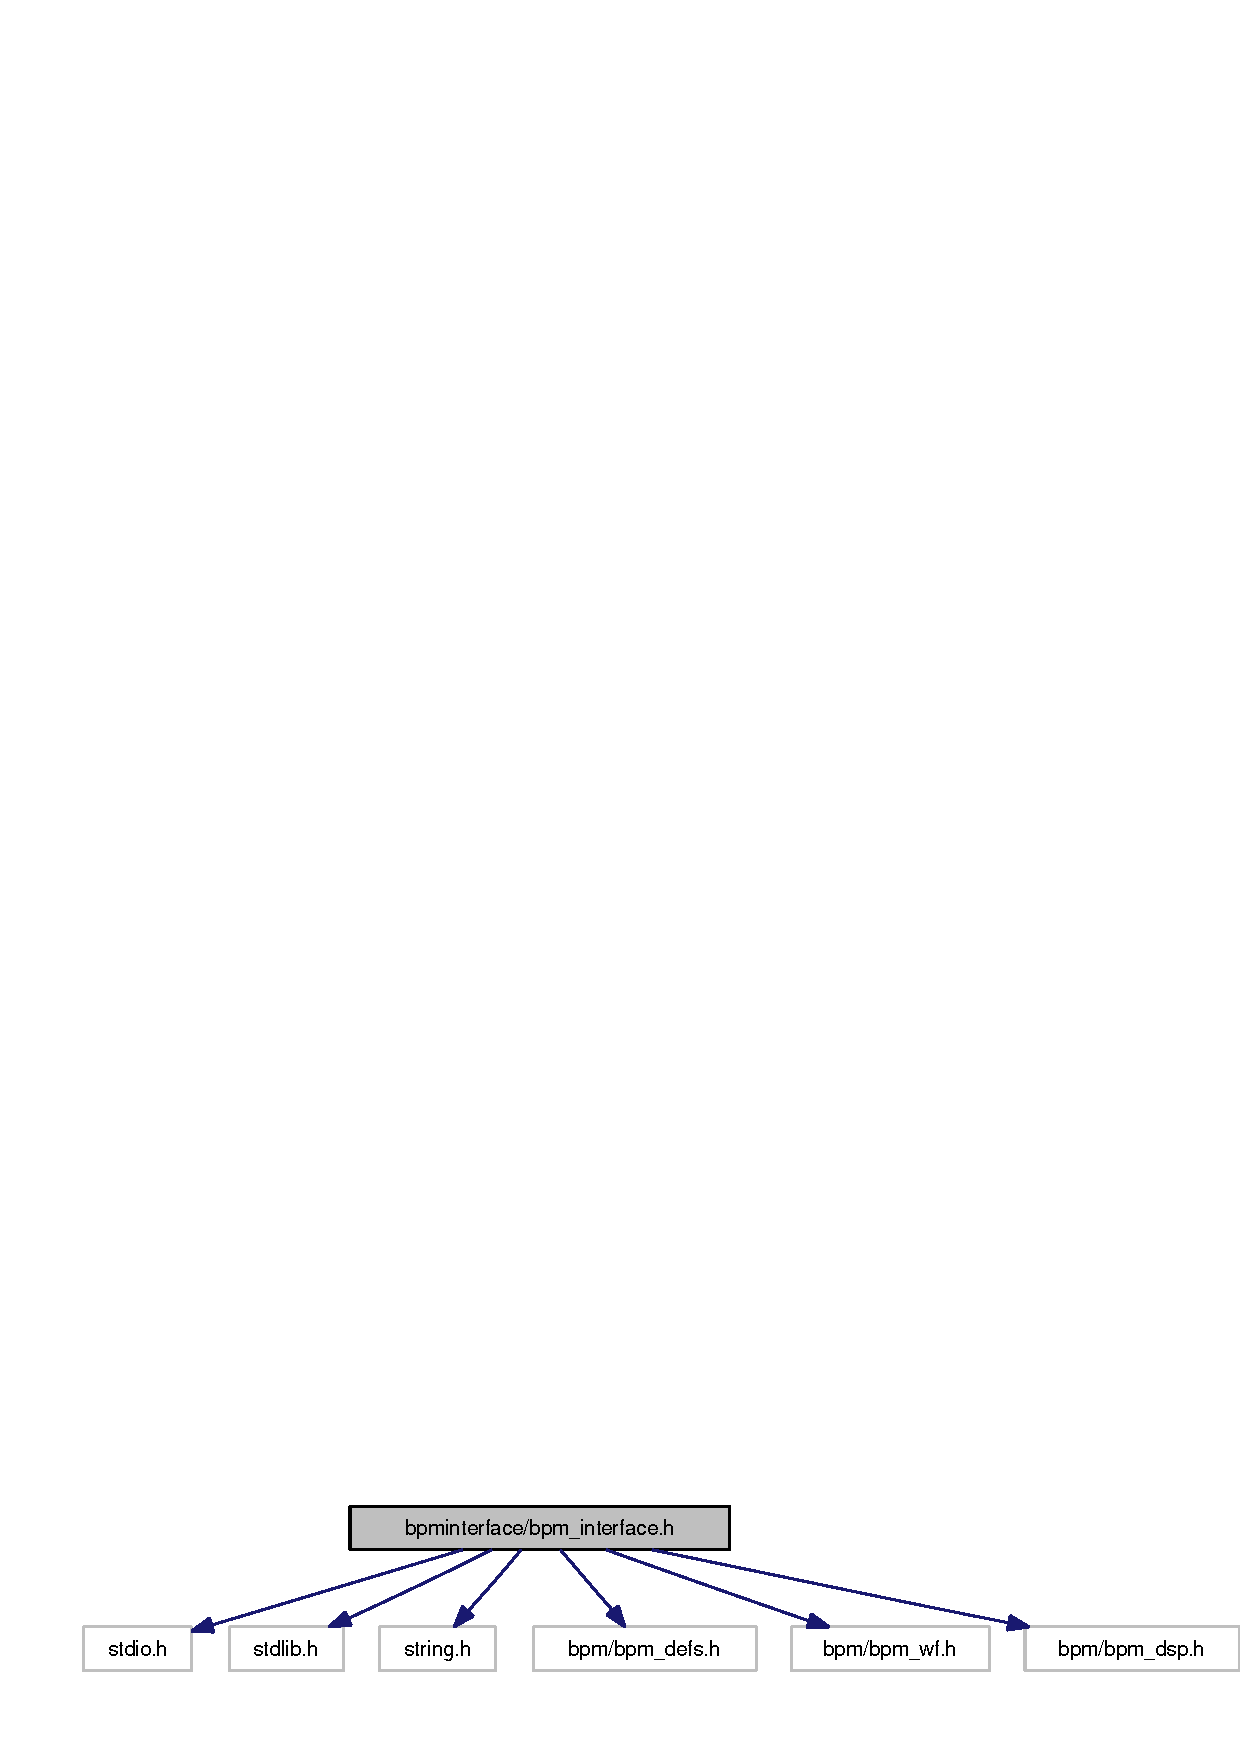
\includegraphics[width=299pt]{bpm__interface_8h__incl}
\end{center}
\end{figure}
\subsubsection*{Data Structures}
\begin{CompactItemize}
\item 
struct {\bf bpmconf}
\item 
struct {\bf bpmcalib}
\item 
struct {\bf bpmproc}
\item 
struct {\bf beamconf}
\item 
struct {\bf bunchconf}
\item 
struct {\bf bpmmode}
\item 
struct {\bf rfmodel}
\end{CompactItemize}
\subsubsection*{Typedefs}
\begin{CompactItemize}
\item 
typedef struct {\bf bpmconf} {\bf bpmconf\_\-t}
\item 
typedef struct {\bf bpmcalib} {\bf bpmcalib\_\-t}
\item 
typedef struct {\bf bpmproc} {\bf bpmproc\_\-t}
\item 
typedef struct {\bf beamconf} {\bf beamconf\_\-t}
\item 
typedef struct {\bf bunchconf} {\bf bunchconf\_\-t}
\item 
typedef struct {\bf bpmmode} \textbf{bpmmode\_\-t}\label{group__interface_g2599c9e0c0e36819170e95dcdcdbdfc0}

\item 
typedef struct {\bf rfmodel} \textbf{rfmodel\_\-t}\label{group__interface_g98c565a46975280f28037fb092e24ec7}

\item 
typedef enum {\bf triggertype} \textbf{triggertype\_\-t}\label{group__interface_gbfc973a0ffff9e74bf9dcdad55ecd3ce}

\end{CompactItemize}
\subsubsection*{Enumerations}
\begin{CompactItemize}
\item 
enum {\bf bpmtype\_\-t} \{ {\bf diode}, 
{\bf monopole}, 
{\bf dipole}
 \}
\item 
enum {\bf triggertype} \{ {\bf positive}, 
{\bf negative}, 
{\bf bipolar}
 \}
\item 
enum {\bf bpmpol\_\-t} \{ {\bf horiz}, 
{\bf vert}
 \}
\item 
enum {\bf bpmphase\_\-t} \{ {\bf randomised}, 
{\bf locked}
 \}
\end{CompactItemize}
\subsubsection*{Variables}
\begin{CompactItemize}
\item 
EXTERN int {\bf bpm\_\-verbose}
\item 
EXTERN int {\bf libbpm\_\-evtnum}
\end{CompactItemize}
